\documentclass[12pt]{article}

\usepackage{a4} 
\usepackage{listings,amsmath,amssymb,graphicx,url,natbib}
\usepackage{color}

\definecolor{dkgreen}{rgb}{0,0.6,0}
\definecolor{gray}{rgb}{0.5,0.5,0.5}
\definecolor{mauve}{rgb}{0.58,0,0.82}

\lstset{frame=tb,
	language=matlab,
	aboveskip=3mm,
	belowskip=3mm,
	showstringspaces=false,
	columns=flexible,
	basicstyle={\small\ttfamily},
	numbers=none,
	numberstyle=\tiny\color{gray},
	keywordstyle=\color{blue},
	commentstyle=\color{dkgreen},
	stringstyle=\color{mauve},
	breaklines=true,
	breakatwhitespace=true,
	tabsize=3
}
\title{Project: Computing the Polar Decomposition}
\author{Xiaobo (Bob) Liu%
        \thanks{%
                School of Mathematics,
                University of Manchester,
                Manchester, M13 9PL, England
                (\texttt{xiaobo.liu@postgrad.manchester.ac.uk}).
               }
}
\date{October 27, 2018}

%%%%%%%%%%%%%%%%%%%%%%%%%%%%%%%%%
\def\R{\mathbb{R}}
\def\C{\mathbb{C}}
\def\nbyn{n \times n}
\def\mbyn{m \times n}
\def\l{\lambda}
\def\norm#1{\|#1\|}      
\def\normi#1{\|#1\|_1}
\def\normo#1{\|#1\|_{\infty}}
\def\Chat{\widehat{C}}
\def\e{eigenvalue}
\def\t#1{\texttt{\upshape #1}}
\DeclareMathOperator{\rank}{rank}
% \DeclareMathOperator{\diag}{diag}   % Requires amsmath.
\def\diag{\mathop{\mathrm{diag}}}     % If not using amsmath.
\def\trace{\mathop{\mathrm{trace}}}   % If not using amsmath.

\def\At{\widetilde{A}}
\def\normt#1{\|#1\|_2}

% Note: this clashes with amsmath.
%\def\bmatrix#1{\left[\matrix{#1}\right]}
% If using amsmath use this instead:
%\makeatletter
%\def\mymatrix#1{\null\,\vcenter{\normalbaselines\m@th
%     \ialign{\hfil$##$\hfil&&\quad\hfil$##$\hfil\crcr
%       \mathstrut\crcr\noalign{\kern-\baselineskip}
%       #1\crcr\mathstrut\crcr\noalign{\kern-\baselineskip}}}\,}
%\makeatother
%\def\bmatrix#1{\left[ \mymatrix{#1} \right]}

% Set up lemma environment and its numbering.
\newtheorem{lemma}{Lemma}[section]

\def\proof{\par{\bf Proof}. \ignorespaces}
\def\qedsymbol{\vbox{\hrule\hbox{%
                     \vrule height1.3ex\hskip0.8ex\vrule}\hrule}}
\def\endproof{\qquad\qedsymbol\medskip\par}

\newtheorem{theorem}{Theorem}
\newtheorem{algorithm}[theorem]{Algorithm}



%%%%%%%%%%%%%%%%%%%%%%%%%%%%%%%%%%%%%%%%%%%%%%%%%%%%%%%%%%%%%%%%%%%%%%%%%%%%
% For fine-tuning spacing in \sqrt etc=.  From \cite[p.~155]{knut99}.
% In math mode, @ will act as a macro that adds 1 unit of space.
% By comparison, \, skips 3mu.

\mathcode`@="8000 % Make @ behave as per catcode 13 (active).  TeXbook p. 155.
{\catcode`\@=\active\gdef@{\mkern1mu}}
%%%%%%%%%%%%%%%%%%%%%%%%%%%%%%%%%%%%%%%%%%%%%%%%
 
%%%%%%%%%%%%%%%%%%%%%%%%%%%%%%%%%%%%%%%%%%%%%%%%%%%%%%%%%%%%%%%%%%%%%%%%%%%%
\newcounter{mylineno}
\makeatletter
\let\oldtabcr\@tabcr
\def\nonumberbreak{\oldtabcr\hspace{3.5pt}}
\def\mynewline{\refstepcounter{mylineno}%
                \llap{\footnotesize\arabic{mylineno}\hspace{5pt}}%
               }
\def\lineref#1{\footnotesize\ref{#1}}
% Next macro adapted from latex.ltx
\gdef\@tabcr{\@stopline \@ifstar{\penalty%
            \@M \@xtabcr}\@xtabcr\mynewline}
\def\myvspace#1{\oldtabcr[#1]\mynewline}
\newenvironment{code}{%
                         % Swap `:' and `colon'...
                         \mathcode`\:="603A  % TeXbook pp 134, 154, 359 (top)
% For original colon     \mathcode`\:="303A  % TeXbook p 344
                         \def\colon{\mathchar"303A}
                         \setcounter{mylineno}{0}
                         \par
                         \upshape
                         \begin{list} % To give indentation
                            {} {\leftmargin = 1cm}
                         \item[]
                         \begin{tabbing}

                         % Default tab stops
                            \hspace*{.3in} \= \hspace*{.3in} \=
                            \hspace*{.3in} \= \hspace*{.3in} \= \kill
                            \mynewline
                        }{\end{tabbing}\end{list}}
\makeatother
%%%%%%%%%%%%%%%%%%%%%%%%%%%%%%%%%%%%%%%%%%%%%%%%%%%%%%%%%%%%%%%%%%%%%%%%%%%%

%%%%%%%%%%%%%%%%
\begin{document}
\maketitle

%%%%%%%%%%%%%%%%%%%%%%
\section*{Tasks}
{\bf Q1.} First, we review the basic theorem of polar decomposition below, which proves useful for later proofs of questions.
\begin{theorem}\label{polardecom}
	(Polar decomposition). Let $A\in\C^{\mbyn}$ with $m\ge n$. There exists a matrix 
	$U\in\C^{\mbyn}$ with orthonormal columns and a unique Hermitian positive 
	semidefinite matrix $H\in\C^{\nbyn}$ such that $A=UH$. The matrix $H$ is given by 
	$(A^*A)^{1/2}$. If $\rank(A)=n$ then $H$ is positive definite and $U$ is 
	uniquely determined.
	
\end{theorem}
\unskip

{\it  Proof} \cite[Chap.~8]{high:FM}.
We can write a singular value decomposition (SVD) of $A$ as 
\begin{equation}
	A=P   \begin{bmatrix}
	\Sigma_r & 0 \\
	0 & 0_{m-r,n-r}
	\end{bmatrix}Q^*
	=
	P \begin{bmatrix}
	I_r & 0 \\
	0 & I_{m-r,n-r}
	\end{bmatrix}Q^*
	\cdot Q
	 \begin{bmatrix}
	\Sigma_r & 0 \\
	0 & 0_{n-r}
	\end{bmatrix}Q^*,
\end{equation}
where $r=\text{rank}(A)$,
$$
P \begin{bmatrix}
I_r & 0 \\
0 & I_{m-r,n-r}
\end{bmatrix}Q^*=:U
$$ 
has orthonormal columns. Also, 
$$
Q\begin{bmatrix}
\Sigma_r & 0 \\
0 & 0_{n-r}
\end{bmatrix}Q^* =:H = \widetilde{Q}^{-1}\begin{bmatrix}
\Sigma_r & 0 \\
0 & 0_{n-r}
\end{bmatrix}\widetilde{Q}\quad (\widetilde{Q}:=Q^*)
$$
is Hermitian positive semidefinite since $H$ and $ \big[ \begin{smallmatrix}
\Sigma_r & 0 \\
0 & 0_{n-r}
\end{smallmatrix}\big] $ are similar, where the later has singular values of $A$ (which are nonnegative) on its diagonal. Then, from 
$A^*A=(UH)^*UH=HU^*UH=H^2$ it follows that $H=(A^*A)^{1/2}$, which uniquely defines $H$. If $r=n$ then $H$ is clearly nonsingular and hence $U=AH^{-1}$ is unique.\endproof
Let $A\in \C^{\mbyn}$ with $m\ge n$ have the QR factorization $A=QR, Q\in \C^{\mbyn}, R\in \C^{\nbyn}$. If $R=UH$ is a polar decomposition then $QU\cdot H$ is a polar decomposition of $A$. This means we can restrict our attention to square matrices since we can always turn the problem of polar decomposition of a rectangular matrix into the one of polar decomposition of a square matrix.
\vspace{.2cm}




\noindent{\bf Q2.} This is obvious from the proof of Theorem \ref{polardecom} above. 
\vspace{.2cm}




\noindent{\bf Q3.} 
{\it  Proof} \cite[Chap.~8]{high:FM}. If $UH=HU$ then, since $U$ is unitary and $H$ is Hermitian, $HU^*=(UH)^*=(HU)^*=U^*H$. Hence, $A^*A=HU^*UH=H^2=HUU^*H=UHHU^*=AA^*$, So $A$ is normal.

If $A^*A=AA^*$ then $H^2=UHHU^*=(UHU^*)UHU^*$. Taking the principal square root of both sides gives $H=UHU^*$, or $HU=UH$, as required. \endproof
\vspace{.2cm}




\noindent{\bf Q4.} Suppose $A=P\Sigma Q^*$ is a SVD of $A$, $\Sigma=\diag(\sigma_1,\sigma_2,\dotsc,\sigma_n)$. Then we have 
$$
\sigma_1\ge \sigma_2\ge \dotsm \ge \sigma_n>0
$$ 
since $A$ is full rank. Also, from previous analysis we know $U=PQ^*$ for $A\in\C^{\nbyn}$. By substitution the formula that we want to verify becomes
$$
PQ^*=\frac{2}{\pi}P\Sigma Q^*\int_{0}^{\infty}(t^2I+Q\Sigma^*\Sigma Q^*)^{-1}\mathrm{d}t.
$$
Premultiplying by $P^*$ gives
\begin{align*} 
  Q^*=&\frac{2}{\pi}\Sigma Q^*\int_{0}^{\infty}(t^2I+Q\Sigma^*\Sigma Q^*)^{-1}\mathrm{d}t	\\
  \Leftrightarrow  \quad
  Q^*=&\frac{2}{\pi}\Sigma\int_{0}^{\infty}(t^2Q+Q\Sigma^*\Sigma)^{-1}\mathrm{d}t	\\
    \Leftrightarrow  \quad
  Q^*=&\frac{2}{\pi}\Sigma\int_{0}^{\infty}(t^2I+\Sigma^2)^{-1}\mathrm{d}tQ^{-1}	\\
\end{align*}
Postmultiplying by $Q$ gives
$$
I=\frac{2}{\pi}\int_{0}^{\infty}\Sigma(t^2I+\Sigma^2)^{-1}\mathrm{d}t,
$$
where the matrix $\Sigma(t^2I+\Sigma^2)^{-1}$ is diagonal. Therefore, the formula that 
we want to verify reduces to 
\begin{equation}\label{svd_int}
1=\frac{2}{\pi}\int_{0}^{\infty}\frac{\sigma_i}{t^2+\sigma_i^2}\mathrm{d}t, \quad 
i=1:n.
\end{equation}
We can prove \eqref{svd_int} for $\sigma_i,\ i=1:n$; let $t=\sigma_i x$, it follows 
the 
right hand side of \eqref{svd_int} becomes
$$
\frac{2}{\pi}\int_{0}^{\infty}\frac{\sigma_i^2}{\sigma_i^2x^2+\sigma_i^2}\mathrm{d}x=
\frac{2}{\pi} \int_{0}^{\infty}\frac{1}{x^2+1}\mathrm{d}x=
\frac{2}{\pi}\cdot \arctan x\big|_{x=0}^{+\infty}=\frac{2}{\pi}\times \frac{\pi}{2}=1.$$ 
\vspace{.2cm}




\noindent{\bf Q5.} Let $X$ be an approximation to $U$, the unitary polar factor of $A$ and write $U=X+E$. Then we have 
\begin{equation}\label{sylvester_eq}
I=U^*U=(X+E)^*(X+E)=X^*X+X^*E+E^*X+E^*E\approx X^*X+X^*E+E^*X
\end{equation}
since $E^*E$ is a second order term in the small perturbation $E$. Then we can rewrite \eqref{sylvester_eq} as 
\begin{equation}\label{skew_hermitian}
X^*E+E^*X = I - X^*X,
\end{equation}
where both sides are Hermitian. We know that any matrix $A$ can be written as the sum of a Hermitian matrix and a skew-Hermitian matrix:
$$
A = \frac{1}{2}(A+A^*) + \frac{1}{2}(A-A^*).
$$
In \eqref{skew_hermitian}, we can calculate the Hermitian part of $X^*E$ and $E^*X$ as $\frac{1}{2}(X^*E+E^*X) = \frac{1}{2}(I - X^*X)$. So, we can assume that $X^*E$ is Hermitian to obtain a feasible solution to equation \eqref{skew_hermitian}. By doing this, \eqref{skew_hermitian} becomes
$$
2X^*E =I - X^*X.
$$
Premultiplying by $\frac{1}{2}X^{-*}$ gives
$
E = \frac{1}{2}(X^{-*}-X),
$
and then $U = X+E = \frac{1}{2}(X^{-*}+X)$, which leads to the Newton's method for computing $U$ if we take $A$ as the initial approximation: 
\begin{equation}\label{Newton_iter}
X_{k+1} = \frac{1}{2}(X_k^{-*}+X_k),\quad X_0=A.
\end{equation}
\vspace{.2cm}




\noindent{\bf Q6.} {\it  Proof}. Firstly, we note that to use Newton's method, $X_0=A$ needs to be of full rank, so here we assume $A$ is nonsingular. Let $A=P\Sigma Q^*$ be an SVD, so we know the unitary polar factor $U=PQ^*$. Next we show by induction that
\begin{equation} \label{indunction}
X_n = PD_nQ^*,
\end{equation}
where 
\begin{equation}\label{signfun}
D_{n+1}= \frac{1}{2}(D_n+D_n^{-1}),\quad D_0=\Sigma.
\end{equation}

{\it Base case:} When $n=1$, $X_1=\frac{1}{2}(X_0^{-*}+X_0)=\frac{1}{2}(A^{-*}+A)$. Substituting $A=P\Sigma Q^*$ into it gives
$$
X_1=\frac{1}{2}((Q\Sigma^* P^*)^{-1}+P\Sigma Q^*)=\frac{1}{2}P(\Sigma+\Sigma^{-1})Q^*
=\frac{1}{2}P(D_0+D_0^{-1})Q^*=PD_1Q^*,
$$
so \eqref{indunction} is true for $n=1$.

{\it Induction step:} Let $k\in\mathbb{N^+}$ be given and  suppose \eqref{indunction} is true for $n = k$. Then 
\begin{align*}
X_{k+1} =& \frac{1}{2}(X_k^{-*}+X_k) \\
  =& \frac{1}{2}((PD_kQ^*)^{-*}+PD_kQ^*) \\
  =& \frac{1}{2}P(D_k^{-1}+D_k)Q^* \\
  =& PD_{k+1}Q^*.
\end{align*}
Thus, \eqref{indunction} holds for $n=k+1$, and the proof of the induction step is complete.

{\it Conclusion:} By the principle of induction, \eqref{indunction} is true for all $n\in \mathbb{N^+}$.

Then we want to prove that the Newton iterates $D_n$ in \eqref{signfun} with nonsingular $D_0=A$ converge quadratically to the matrix sign function $S=\text{sign}(A)$.

We know if $A$ has eigenvalues $\lambda_1,\lambda_2,\dotsc$, then eigenvalues of $A^{-1}$ are $\lambda_1^{-1},\lambda_2^{-1},\dotsc$. For $\lambda=re^{i\theta}$ we have $\lambda+\lambda^{-1}=(r+r^{-1})\cos\theta+i(r-r^{-1}\sin\theta)$, and hence eigenvalues of $D_n$ remain in their open half-plane under the mapping \eqref{signfun}. Hence, $D_n$ is well-defined and nonsingular for all $n$. Then according to the definition of matrix sign function by Jordan canonical form, it is easy to see sign$(D_n)=\text{sign}(D_0)=\text{sign}(A)=S$. Therefore, $D_n+S=D_n+\text{sign}(D_n)$ is also nonsingular from the view of their eigenvalues.

Also, we see $D_n$ are rational functions of $D_0=A$ and hence, like $A$, commute with $\text{Sign}(A)=S$, then we have 
\begin{align} \label{D_n}
D_{n+1}\pm S &= \frac{1}{2}(D_n+D_n^{-1}\pm 2S)  \nonumber \\
&= \frac{1}{2}D_n^{-1}(D_n^2\pm 2D_nS+ I) \nonumber\\
&= \frac{1}{2}D_n^{-1}(D_n\pm S)^2, 
\end{align}
and hence
\begin{align*}
(D_{n+1}- S)(D_{n+1}+ S)^{-1} &= \frac{1}{2}D_n^{-1}(D_n- S)^2 \cdot
2(D_n+S)^{-2}D_n \\
&= (D_n- S)^2(D_n+S)^{-2} \\
&= ((D_n- S)(D_n+S)^{-1})^2.
\end{align*}
If we define 
\begin{equation}\label{def_Gk}
G_n=(D_n- S)(D_n+S)^{-1},
\end{equation}
we have $G_{n+1}=G_{n}^2=\dotsm=G_{0}^{2^{n+1}}$. Now $G_0=(D_0-S)(D_0+S)^{-1}=(A-S)(A+S)^{-1}$ has eigenvalues $(\lambda-\text{sign}(\lambda))/(\lambda+\text{sign}(\lambda))$, where $\lambda\in \Lambda(A)$. It follows the eigenvalues of $G_0$ lie inside the unit circle since $\lambda$ is not pure imaginary, which means $\rho(G_0)<1$, then $G_n=G_{0}^{2^{n}}\to 0$ as $n\to \infty$. Hence from \eqref{def_Gk} we have
$$
D_n= (I-G_n)^{-1}(I+G_n)S \to S \quad \text{as} \ n\to\infty. 
$$
Finally, taking norms in \eqref{D_n} with the minus sign gives 
$$
\norm{D_{n+1}-S}=\frac{1}{2} \norm{D_n^{-1}(D_n - S)^2}\le
\frac{1}{2} \norm{D_n^{-1}}\norm{D_n - S}^2,
$$
which displays the quadratic rate of convergence.

Above all, we have proved that the Newton iterates $X_n$ for computing $U$ are equivalently $X_n = PD_nQ^*$, where $P$ and $Q$ are given, and $D_n$ with $D_0=\Sigma$ converge quadratically to the matrix sign function $\text{sign}(\Sigma)=I$. Hence we can deduce that $X_n$ converge quadratically to $PIQ^*=PQ^*=U$. \endproof
\vspace{.2cm}




\noindent{\bf Q7.} The Newton--Schulz iteration for computing $U$ is written as
\begin{equation} \label{Newton--Schulz_iter}
X_{k+1}=\frac{1}{2}X_k(3I-X_k^*X_k), \quad X_0=A.
\end{equation}
In Newton's method, there is a need for computing the inverse of matrices, which can make the cost of this method exorbitant. One way to avoid this (and hence use only matrix multiplication) is to approximate it by one step of Newton's method for matrix inverse, say, for computing $A^{-1}$ \cite[Chap.~5]{high:FM}:
$$
X_{k+1} = X_k(2I-AX_k).
$$
Then using this formula we can remove the matrix inverse from the Newton iteration \eqref{Newton_iter} to obtain the Newton--Schulz iteration \eqref{Newton--Schulz_iter} for computing $U$.

First, we note that to use Newton--Schulz method, $X_0=A$ needs to be of full rank, so here we assume $A$ is nonsingular. Let $A=P\Sigma Q^*$ be an SVD, so we know the unitary polar factor $U=PQ^*$. Next we show by induction that
\begin{equation} \label{indunction_2}
X_k = P\Sigma_kQ^*,
\end{equation}
where 
\begin{equation}\label{ns_2}
\Sigma_{k+1}= \frac{1}{2}(3\Sigma_k-\Sigma_k^{3}),\quad \Sigma_0=\Sigma.
\end{equation}

{\it Base case:} When $k=1$, $X_1=\frac{1}{2}X_0(3I-X_0^*X_0)=\frac{1}{2}A(3I-A^*A)$. Substituting $A=P\Sigma Q^*=P\Sigma_0 Q^*$ into it gives
\begin{align*}
X_1&=\frac{1}{2}P\Sigma_0 Q^*(3I-(P\Sigma_0 Q^*)^*P\Sigma_0 Q^*) \\
&=\frac{1}{2}(3P\Sigma_0 Q^*-P\Sigma_0^3 Q^*) \\
&=P\cdot\frac{1}{2}(3\Sigma_0 -\Sigma_0^3)\cdot Q^* \\
&=P\Sigma_1Q^*,
\end{align*}
so \eqref{indunction_2} is true for $k=1$.

{\it Induction step:} Let $s\in\mathbb{N^+}$ be given and  suppose \eqref{indunction_2} is true for $k = s$. Then 
\begin{align*}
X_{s+1} &= \frac{1}{2}X_s(3I-X_s^*X_s) \\
&=\frac{1}{2}P\Sigma_s Q^*(3I-(P\Sigma_s Q^*)^*P\Sigma_s Q^*) \\
&=\frac{1}{2}(3P\Sigma_s Q^*-P\Sigma_s^3 Q^*) \\
&=P\cdot\frac{1}{2}(3\Sigma_s -\Sigma_s^3)\cdot Q^* \\
&=P\Sigma_{s+1}Q^*
\end{align*}
Thus, \eqref{indunction_2} holds for $k=s+1$, and the proof of the induction step is complete.

{\it Conclusion:} By the principle of induction, \eqref{indunction_2} is true for all $n\in \mathbb{N^+}$.

Now we want to find the conditions for $\Sigma_0=\Sigma$ such that the map \eqref{ns_2} converges to the identity matrix, then $X_{k}$ converges to $PQ^*=U$. It is obvious that $\Sigma_k$ are diagonal. According to the assumption $A$ is nonsingular, we know the diagonal elements of $\Sigma$: $\sigma_1=\norm{A}_2>\sigma_2>\dotsm>\sigma_n$ are strictly positive. Therefore, we consider the scalar map with $k=0,1,\dotsc$:
\begin{equation}\label{scalar_map}
x_{k+1}=f(x_k)=\frac{1}{2}x_k(3-x_k^2), \quad x_0>0.
\end{equation}
By solving $x=\frac{1}{2}x(3-x^2)$ we obtain the only fixed point of this map in $(0,+\infty)$ is $x= 1$. Then we plot the graph of the function (map) as below.
\begin{figure}[h]
	\centering
	\includegraphics[width=.6\textwidth]{function.eps}
\end{figure}

It is easy to compute that $f(0)=0$, $f(\sqrt{3})=0$, and $f(1)=1$, which is the 
maximum of $f$ in $(0,+\infty)$. Also, $f'(x)>0$ for $0<x<1$, and $f'(x)<0$ for 
$1<x<\sqrt{3}$. Hence, $0<f(x)<1$ for $x\in(0,\sqrt{3})$. If we write
$$
x_{k+1}=x_k(1+\frac{1}{2}(1-x_k^2)),
$$
we see immediately $x_{k+1}>x_k$ for $x_k\in (0,1)$. It follows that $x_k\to f(1)=1$ as $k\to \infty$ for $x_0\in (0,\sqrt{3})$. For $x_0>\sqrt{3}$, even though the monotonic decrease of $f$ can simplify the problem, the cases become much more complicated. For example, it is can be shown in a similar way that $f(f(2))=f(-1)=-1$, and thus $x_k\to f(-1)=-1$ as $k\to \infty$ for $x_0\in (\sqrt{3},2)$. Furthermore, let
\begin{equation}\label{numerical}
f(f(m_1))=f(-\sqrt{3})=0, \quad f(f(m_2))=\sqrt{3}
\end{equation}
for $m_2>m_1>2$, then it is not hard to see that for $x_0\in (m_1,m_2)$, $x_k\to 1$ as $k\to \infty$. Numerically solving \eqref{numerical} by MATLAB, we obtain $m_1\approx2.1478, m_2\approx2.2212$, so we can assert for $x_0\in (2.15,2.22)$, $x_k\to 1$ as $k\to \infty$. By solving $-x=f(x)=\frac{1}{2}x(3-x^2)$ we obtain $x=\pm \sqrt{5}$. Actually, if we consider more iterations of the map $f$, there are infinitely many such intervals $(a,b)\subset(\sqrt{3},\sqrt{5})$ on which if the starting point $x_0$ lies then $x_k\to 1$ as $k\to \infty$. However, the later results are hard to be practically exploited since the requirements are on all singular values of the matrix $A$. Besides, if we write \eqref{scalar_map} as 
$$
x_{k+1}-1 = -\frac{1}{2}(x_k^3-2x_k^2+x_k+2x_k^2-4x_k+2)
=-\frac{1}{2}(x_k-1)^2(x_k+2),
$$
which leads to 
$$
\norm{x_{k+1}-U}\le \frac{1}{2}\norm{x_{k}-U}^2\norm{x_{k}+2U}
$$
by taking norms on both sides, which displays the quadratic rate of convergence. Hence, we conclude that in the Newton--Schulz iteration \eqref{Newton--Schulz_iter}, $X_k\to U$ quadratically as $k\to\infty$ if $\norm{A}_2<3$.
 \vspace{.2cm}
 
 

\noindent{\bf Q8.} For the Newton's method: $X_{k+1} = \frac{1}{2}(X_k^{-*}+X_k),\ X_0=A$, the computational cost mainly comes from the matrix inversion since it only requires one matrix inversion and one matrix addition in matrix level. To compute $X_k^{-1}$ for a given $X_k$, we form $X_kX_k^{-1}=I$ and solve the linear systems $X_kX_{ki}^{-1}=e_i,\ i=1:n$ using the $PA=LU$, the LU factorization with permutation that requires $\frac{2}{3}n^3+\mathcal{O}(n^2)$ flops. Then we have $n$ upper triangular systems and $n$ lower triangular systems to solve, where the right-hand side vector $e_i$ has $i-1$ leading zeros. Exploiting this, we can reduce the flops to $\frac{1}{3}n^3+n^3+\mathcal{O}(n^2)=\frac{4}{3}n^3+\mathcal{O}(n^2)$ from $2n^3+\mathcal{O}(n^2)$ that would be required for solving $2n$ general triangular systems. Hence, the total cost of one step of Newton's method is essentially $\frac{2}{3}n^3+\frac{4}{3}n^3=2n^3$ flops. 

The Newton--Schulz iteration can be written as: $X_{k+1}=\frac{1}{2}(3X_k-X_kX_k^*X_k),\ X_0=A$, the computational cost mainly comes from the two matrix multiplications of forming $X_kX_k^*X_k$. We can exploit the symmetry of the product of $X_kX_k^*$ to reduce the cost of computing it to $n^3+\mathcal{O}(n^2)$ flops. Then we compute the second matrix multiplication $(X_kX_k^*)X_k$ in the general way, which requires $2n^3+\mathcal{O}(n^2)$ flops. Therefore, the total cost of one step of Newton--Schulz iteration is essentially $n^3+2n^3=3n^3$ flops.

Ignoring operation counts, from the results above we see immediately that matrix multiplication has to be at least $3n^3/2n^3=1.5$ times faster than matrix inversion for Newton--Schulz to be faster than Newton.
 \vspace{.2cm}



\noindent{\bf Q9.} The link to my GitHub repository: \verb|https://github.com/Xiaobo-Liu/polar_decom|. 

The algorithm computes the polar decomposition $A = UH$ of $A\in\C^{\nbyn}$ (ideally, $A$ should be nonsingular), which uses the methods we have discussed before to compute the unitary polar factor $U$, and then it easily computes the Hermitian factor $H$ by just one matrix multiplication $H = U^*A$.


Let us assume $A$ is nonsingular. First, from our previous proofs, we have shown that 
the Newton's method is bound to quadratically converge to the unique polar factor $U$, 
while the quadratic convergence of Newton--Schulz method is subject to the condition 
that $\norm{A}_2<3$. Because matrix multiplication is very fast on high-performance 
computers compared with matrix inversion, the algorithm will start with Newton 
iteration and switch to the Newton--Schulz iteration when the later is certain to 
converge, to ensure the convergence and to some degree optimize the speed. Based on 
this, we could use the criteria 
$$
\norm{X_k}_2 < \sqrt{3}
$$
to judge when the algorithm switch to the Newton--Schulz iteration (we have tried using this criteria, in which case it makes no big difference to the iterations required). Alternatively, we chose to use 
\begin{equation} \label{criteria}
\norm{I-X_k^*{X_k}}\le \theta
\end{equation}
for some $\theta <1$, where we think $\norm{I-X_k^*{X_k}}$ can be viewed as a measure of unitarity of $X_k$. It is not hard to show (as shown in \cite{hisc90}) that if $\theta<1$ for certain $X_k$, then $\norm{I-X_k^*{X_k}}$ is strictly decreasing if the Newton--Schulz iteration is employed. In the algorithm, we used $\theta=0.6$ as suggested in \cite{hisc90}. Also, it is shown in \cite[Lem.~8.17]{high:FM} that
\begin{equation} \label{lemma}
\frac{\norm{A^*A-I}}{1+\sigma_1(A)}\le \norm{A-U} \le \frac{\norm{A^*A-I}}{1+\sigma_n(A)},
\end{equation}
for any unitarily invariant norm. This inequality \eqref{lemma} shows the measure of the distance $\norm{X_k^*{X_k}-I}$ is essentially equivalent to the measure of the forward error $\norm{X_k-U}$, even if we are using the infinity norm to measure $\norm{X_k^*{X_k}-I}$ due to the norm equivalence of matrices between the 2-norm and the infinity norm
$$
\frac{1}{\sqrt{n}}\norm{A}_\infty\le\norm{A}_2\le\sqrt{n}\norm{A}_\infty.
$$

The discussion above validates the convergence of the algorithm which combines the Newton's iteration and the Newton--Schulz iteration. On each iteration we will also print out $\norm{I-X_k^*{X_k}}_\infty$ and $\norm{X_k-X_{k-1}}_\infty/\norm{X_k}_\infty$, the normwise relative distance between two iterates, which reveals the `movement' we make during each iteration. Finally, we will terminate the algorithm only when $\norm{X_k-X_{k-1}}_\infty/\norm{X_k}_\infty$ becomes less than the tolerance that we choose as $10u$ (here $u$ is the unit roundoff), that is to say, when further progress that we can make becomes rather limited. Below the Table \ref{table} lists the results on five kinds of test matrices that we used. In Appendix A, we plot $RD_k$ and $EFE_k$ on each iteration for the matrices. 

\begin{table}[ht]

	\begin{center}
				\caption{Results on test matrices. We set 
				$RD_k:=\norm{X_k-X_{k-1}}_\infty/\norm{X_k}_\infty$, 
				$EFE_k:=\norm{I-X_k^*{X_k}}_\infty$, and $k$ to be the total 
				iterations. IS denotes the first iteration that the algorithm switch 
				to the Newton--Schulz method. The reference `exact' polar factor 
				$\widehat{U}$ is computed in quadruple precision.}
		\begin{tabular}{lllllll} 
			\hline
			 $A$ & $\kappa_\infty(A)$ &  $k$ & IS & $RD_k$  & $EFE_k$ &  
			 $\norm{\widehat{U}-X_k}_\infty$ \\
			\hline
		    \t{randn(5)} &  28.39 & 9 & 4 & 1.57$\times 10^{-16}$ & 5.89$\times 
		    10^{-16}$ &  6.20$\times 10^{-16}$   \\
		   \t{randn(20)} & 744.16 & 10 & 6 & 2.55$\times 10^{-16}$ & 1.24$\times 
		   10^{-15}$ & 1.98$\times 10^{-15}$ \\
		   \t{randn(100)}& 1.97$\times 10^{3}$ &10 & 6&  5.77$\times 10^{-16}$& 
		   4.26$\times 10^{-15}$ & 1.60$\times 10^{-14}$ \\
		   \t{eye(8)}    & 1 & 1 & NA & NA&  0 & 0 \\
		   \t{hilb(6)}   & 2.91$\times 10^{7}$& 29 & 25 & 1.12$\times 10^{-16}$ & 1.34$\times 10^{-27}$ & 9.37$\times 10^{-12}$ \\
		   \t{magic(6)}  & 5.00$\times 10^{17}$& 58 & 54 & 1.46$\times 10^{-16}$ & 
		   4.10$\times 10^{-16}$ & 1.29$\times 10^{-2}$ \\
		   \t{hadamard(8)} &  8 & 8 & 3 & 1.77$\times 10^{-16}$ &  6.39$\times 
		   10^{-16}$ & 4.30$\times 10^{-16}$ \\	
			\hline		
		\end{tabular}
		\label{table}
	\end{center}
\end{table}

Some observations on the results:
\begin{enumerate}
\item For random matrices \t{randn(n)}, the performance of our algorithm is generally good. When the condition number grows as the size of the matrix increases, it tends to require more iterations. Also, it shows that $\norm{I-X_k^*{X_k}}_\infty$ is a good indicator of the forward error $\norm{U-X_k}_\infty$ in these cases.
\item For the identity matrix, the algorithm exactly converges to the $U$ we want with one iteration. From the view of polar decomposition of the identity $I=I\cdot I$, this is not surprising because the initial matrix that we starts with in the Newton method is the $U$ we want to compute.
\item For \t{hilb(6)}, it takes distinctly more iterations than previous matrices for the algorithm to reach its stopping criteria. From its profiles of $\norm{X_k-X_{k-1}}_\infty/\norm{X_k}_\infty$ and $\norm{I-X_k^*{X_k}}_\infty$ in Appendix A, we see the convergence of the Newton method is much slower than that of the Newton--Schulz method. Also, we note that the result is still accurate given that the condition number is of order $10^7$.
\item \t{magic(6)} is a singular matrix, which becomes numerically invertible in MATLAB due to the occurrence of rounding errors. In this case it takes the algorithm 58 iterations to converge. Again, from its profiles of $\norm{X_k-X_{k-1}}_\infty/\norm{X_k}_\infty$ and $\norm{I-X_k^*{X_k}}_\infty$, we see the convergence of the Newton method is very slow because matrix inversion is required in its iterations. We also note that the forward error of the result is considerably big and much larger than $\norm{I-X_k^*{X_k}}_\infty$.
\item For the well-conditioned matrix \t{hadamard(8)}, it only takes 8  iterations to converge.
\item To summarize, it tends to require more iterations for the algorithm to converge 
when the condition number of the computed matrix grows. Generally, 
$\norm{I-X_k^*{X_k}}_\infty$ is a good indicator of the forward error 
$\norm{U-X_k}_\infty$ for nonsingular matrices, while for singular matrices it may not 
be. Finally, our algorithm is not a good choice for singular matrices in terms of 
accuracy and speed.
\end{enumerate}
 \vspace{.2cm}
 
 
\noindent{\bf Q10.} For a symmetric positive definite matrix $A$, if we firstly factorise $A$ using a Cholesky decomposition: $A=R^*R$, and then we compute a polar decomposition of the Cholesky factor $R=UH$, then we will obtain
$$
A=R^*R=(UH)^*(UH)=H^*U^*UH=H^*H=H^2,
$$
where by definition $H$ is the square root of $A$. Using this idea, we write a function \t{plosqrt(A)} that computes the square root of a symmetric positive definite matrix $A$.


\bibliographystyle{plain}
\bibliography{pdbib}{}
\appendix
\clearpage
\section*{Appendix A: Figures}

\begin{figure}[h]
	\centering
	\caption{$RD_k$ and $EFE_k$ on each iteration for \t{randn(5)}}
	\includegraphics[width=.67\textwidth]{randn5.eps}
\end{figure}


\begin{figure}[h]
	\centering
	\caption{$RD_k$ and $EFE_k$ on each iteration for \t{randn(20)}}
	\includegraphics[width=.67\textwidth]{randn20.eps}
\end{figure}

\begin{figure}[h]
	\centering
	\caption{$RD_k$ and $EFE_k$ on each iteration for \t{randn(100)}}
	\includegraphics[width=.7\textwidth]{randn100.eps}
\end{figure}

\begin{figure}[h]
	\centering
	\caption{$RD_k$ and $EFE_k$ on each iteration for \t{hilb(6)}}
	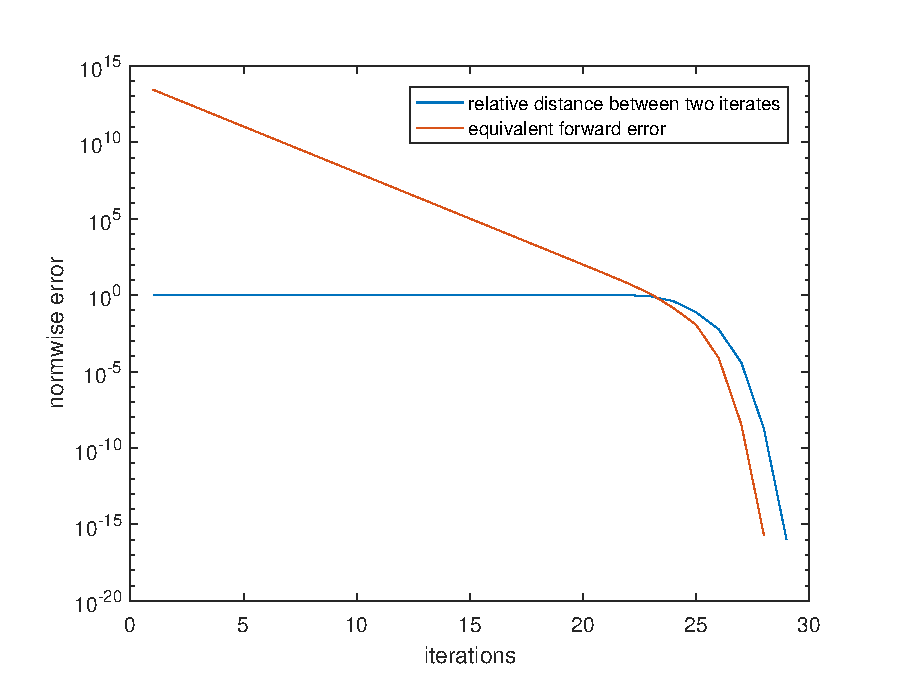
\includegraphics[width=.7\textwidth]{hilb6.eps}
\end{figure}

\begin{figure}[h]
	\centering
	\caption{$RD_k$ and $EFE_k$ on each iteration for \t{magic(6)}}
	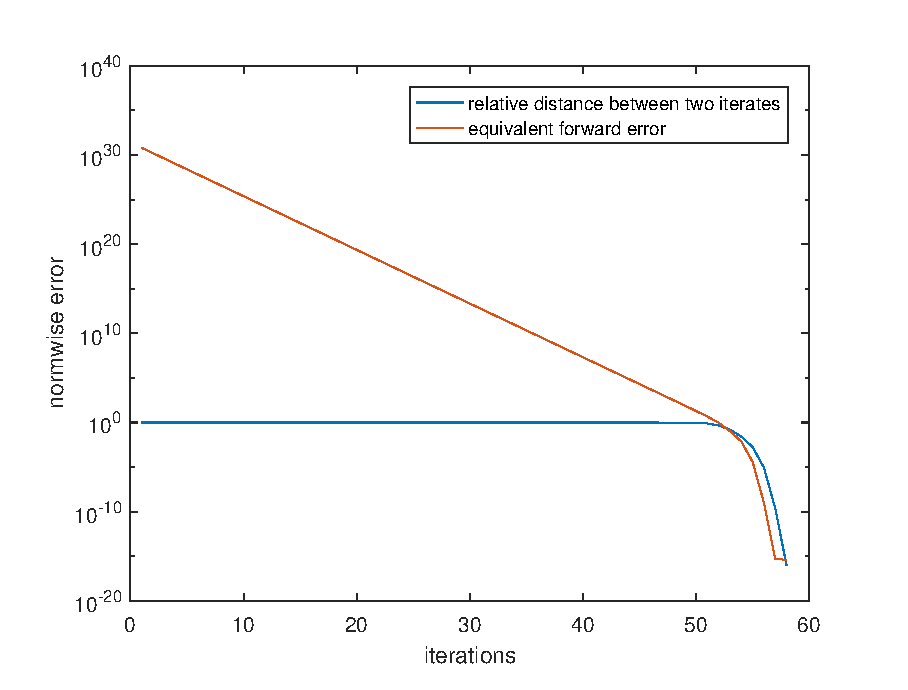
\includegraphics[width=.7\textwidth]{magic6.eps}
\end{figure}

\begin{figure}[h]
	\centering
	\caption{$RD_k$ and $EFE_k$ on each iteration for \t{hadamard(8)}}
	\includegraphics[width=.7\textwidth]{hadamard8.eps}
\end{figure}
\clearpage
\section*{Appendix B: MATLAB Code}
\begin{lstlisting}
function [U, H, its] = poldec(A)
%POLDEC Polar decomposition
%   [U, H, its] = poldec(A) computes the polar decomposition A = U*H of the
%   square, nonsingular matrix A. ITS is the number of iterations for
%   convergence.

% Setting the parameters which can be changed if necessary
tol = 10*eps; % convergence tolerance: of order of the unit roundoff
theta = 0.6;  % switch tolerance
plots = true; % plot the errors against iterations

validateattributes(A, {'double', 'single'}, {'square'});
n = length(A);
X_prev = A;
I = eye(n);
its = 0;
terminates = false;
switches = false;
notice = false; % give a notice when switches
if plots	% I will avoid opening a file to store data in the future
	fid = fopen('data.txt','w'); % store data into data.txt for plotting
end
while terminates == false
	its = its + 1;
	if ~switches % Newton method
		X_next = (X_prev + inv(X_prev)')/2;
		CP = X_next'*X_next;	% store and reuse this value
		% compute the normwise relative distance (RD) between two
		% iterates and the equivalent forward error (FE)
		RD = norm(X_next - X_prev, Inf)/norm(X_next, Inf);
		EFE = norm(I - CP, Inf);
		if EFE <= theta
			switches = true;
			notice = true;
		end
	else % switch to Newton-Schulz method
		X_next = (3*X_prev - X_prev*CP)/2;
		CP = X_next'*X_next;
		RD = norm(X_next - X_prev, Inf)/norm(X_next, Inf);
		EFE = norm(I - CP, Inf);   
	end
	if plots
		fprintf(fid, '%.2d %.16f %.16f \n', its, RD, EFE);
	end
	fprintf('%.2dth iters: Relative Distance %.4e, Forward Error %.4e \n', its 
	, RD,EFE);
	if notice
		fprintf(' Now switch from the Newton iteration to the Newton-Schulz 
		iteration.\n');
		notice = false; % only one notice is needed
	end
	if RD < tol
		terminates = true;
		if plots
			fclose(fid);
		end
	end
	X_prev = X_next;
end
U = X_prev;
H = U'*A;
H = (H' + H)/2; % Force Hermitian by taking nearest Hermitian matrix

% load data and plot the errors
if plots
	data = load('data.txt');
	semilogy(data(:,1),data(:,2),data(:,1),data(:,3));
	legend('relative distance between two iterates','equivalent forward error');
	xlabel('iterations');
	ylabel('normwise error');
end
end
\end{lstlisting}
\vspace{1cm}
\begin{lstlisting}
function S = plosqrt(A)
%POLSQRT Matrix square root
%   S = plosqrt(A) Computes the square root S = A^(1/2) of the symmetric
%   positive definite matrix A by doing a Cholesky decomposition and
%   calling poldec.

[R, p] = chol(A);
if p~= 0
	disp('sorry, I only work for a sym.pos.def matrix.');
else
	[~, S] = poldec(R);
	clc; % clear the displays that result from calling poldec()
	disp('>> plosqrt()');
end
end


\end{lstlisting}
\end{document}
